\section{Développement du circuit-imprimé} \label{sec:Dev-PCB}
Dans cette section, nous nous attarderons sur le processus de conception et de développement du \gls{pcb}. Nous aborderons également les différents aspects mécanique d'intégration du projet, en essayant d'analyser les différentes contraintes des composants et la structure globale. Cette analyse combinée des aspects électroniques et mécaniques est cruciale pour assurer la réussite du projet.

\clearpage

\subsection{Mécanique du projet} \label{ssec:mechProjet}
L'un des objectifs majeurs du projet est de concevoir un produit qui, par sa petite taille et son design compact, se prête à une installation qui se veut à la fois discrète et non encombrante.
 
\subsubsection{Choix du boitier}
Pour réduire la taille au maximum, un processus itératif a eu lieu, consistant à trouver un boîter plastique le plus petit possible et d'essayer en respectant les contraintes de taille, de placer les composants, puis, d'observer et déduire si la taille est suffisante. Grâce à cette procédure itérative, un boîtier a été déterminé : le \fbox{\textbf{SIC5-9-3B}} de chez \href{https://www.takachi-enclosure.com/products/SIC}{TAKACHI}.

\begin{figure}[h!]
	\centering
	\begin{subfigure}[b]{0.6\textwidth}
		\centering
		\includegraphics[width=\textwidth]{../figures/dev-pcb/boitier-dim}
		\caption{Dimensions boîtier}
		\label{fig:boitier-dim}
	\end{subfigure}
	\hfill
	\begin{subfigure}[b]{0.35\textwidth}
		\centering
		\includegraphics[width=\textwidth]{../figures/dev-pcb/boitier-dims-pcb}
		\caption{Dimension trous \gls{pcb}}
		\label{fig:boitier-dims-pcb}
	\end{subfigure}
	\caption{Dimensions du SIC5-9-3B}
	\source{\href{https://www.takachi-enclosure.com/products/SIC}{\Gls{datasheet} du SIC5-9-3B, TAKACHI}}
	\label{fig:boitier-dimensions}
\end{figure}

\subsubsection{Placement des composants} \label{ssec:placementComp}
Désormais, sachant que nous connaissons les dimensions du \gls{pcb} grâce à la figure \ref{fig:boitier-dims-pcb}, nous pouvons positionner les composants de manière optimisée pour le routage et la mécanique. En prenant différents éléments en compte :

\begin{table}[!h]
\begin{adjustbox}{max width=\textwidth}
	\begin{tabular}{llll}
	\hline
	& Élément & & Contraintes, règles et dispositions particulières \\
	\hline
	\faChevronRight & \textbf{Connecteur USB} & : & Placer proche du bord, usinage du boitier pour passer chargeur. \\
	\faChevronRight & \textbf{Connecteur \micro SD} & : & Proche du bord, facile d'accès. \\
	\faChevronRight & \textbf{\gls{gnss}} & : & Isolé des autres composants, faciliter réception. \\
	\faChevronRight & \textbf{Carte BNO055} & : & Espace requis, permettre de le braser sur le \gls{pcb}. \\
	\faChevronRight & \textbf{LED de vie} & : & Dégagée, peut être déportée avec un guide-lumière. \\
	\faChevronRight & \textbf{Connecteur batterie} & : & Accessible et permettre de passer les fils de l'autre coté du \gls{pcb}. \\
	\faChevronRight & \textbf{Connecteur bouton ON/OFF} & : & Bouton déporté sur le boîtier. \\
	\faChevronRight & \textbf{Bouton reset} & : & Accessible pendant le développement et en cas de bug. \\
	\end{tabular}	
\end{adjustbox}
\label{tab:reglesPlacement}
\caption{Tableau des contraintes de placement}
\source{Auteur}
\end{table}

\clearpage

\begin{figure}[h]
	\centering
	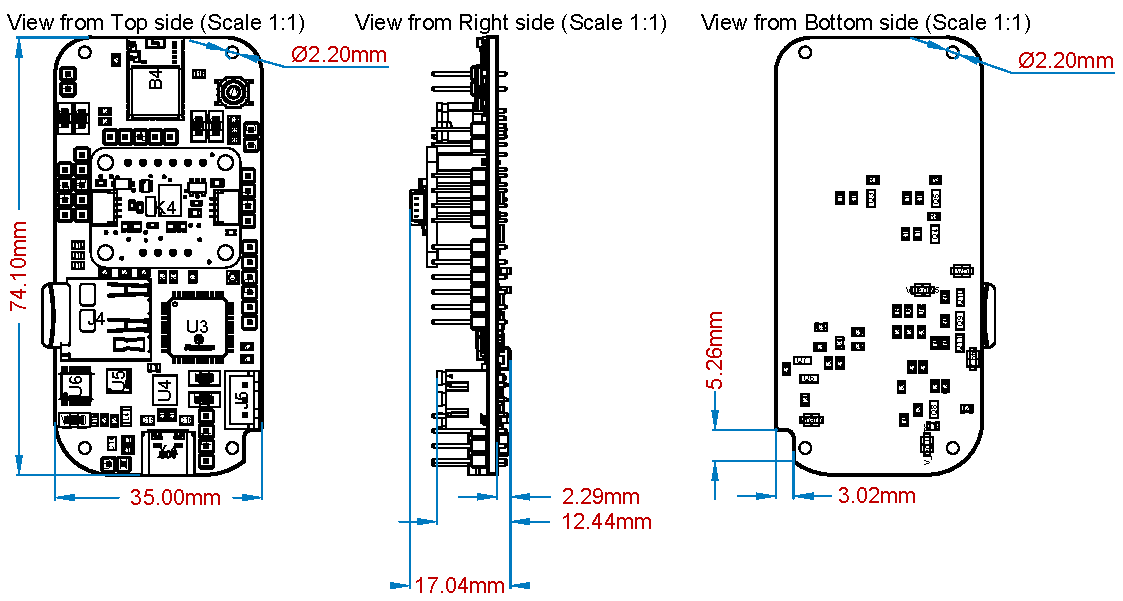
\includegraphics[width=1\linewidth]{../figures/dev-pcb/PCB-Dims}
	\caption{Placement des composant et dimensions de la carte}
	\label{fig:pcb-dims}
\end{figure}

En considérant les éléments de la table \ref{tab:reglesPlacement}, nous obtenons un design tel que la figure \ref{fig:pcb-dims}

\clearpage

\subsection{Bill of materials} \label{ssec:BOM}
Avec le schéma et la mécanique désormais établis, il est possible de dresser une liste des composants. La table \ref{tab:BOM_PRIX} présente une liste des composants \textbf{hors-stock} qui ont été commandés auprès de différents distributeurs. Quant à la table \ref{tab:BOM-Stock}, elle détaille les composants actuellement \textbf{en stock} dans les locaux de l'école supérieure, ainsi que leurs prix. Ces derniers n'ont pas été commandés. Les tableaux \ref{tab:Bom_resistors} et \ref{tab:Bom_Capa}, présentent les valeurs des résistance et condensateurs utilisées dans le projet.

\begin{table}[h]
	\centering
	\resizebox{\textwidth}{!}{%
		\begin{tabular}{|l|llll|}
			\hline
			Composant                            & \multicolumn{1}{l|}{Fournisseur} & \multicolumn{1}{l|}{Réference}              & \multicolumn{1}{l|}{Quantité} & Prix [CHF] \\ \hline
			Batterie PICPAL36                    & \multicolumn{1}{l|}{Farnell}     & \multicolumn{1}{l|}{PICPAL36}               & \multicolumn{1}{l|}{1}        & 36,54      \\ \hline
			BNO055-Adafruit                      & \multicolumn{1}{l|}{Digikey}     & \multicolumn{1}{l|}{1528-4646-ND}           & \multicolumn{1}{l|}{1}        & 26,06      \\ \hline
			GNSS                                 & \multicolumn{1}{l|}{Digikey}     & \multicolumn{1}{l|}{672-CAM-M8C-0CT-ND}     & \multicolumn{1}{l|}{1}        & 23,49      \\ \hline
			Boitier boite noire                  & \multicolumn{1}{l|}{Farnell}     & \multicolumn{1}{l|}{CHH9840BK}              & \multicolumn{1}{l|}{1}        & 6,84       \\ \hline
			Guide lumière &
			\multicolumn{1}{l|}{Digikey} &
			\multicolumn{1}{l|}{\begin{tabular}[c]{@{}l@{}}LFB075CTP-ND\\ 492-1980-ND\end{tabular}} &
			\multicolumn{1}{l|}{4} &
			6,13 \\ \hline
			PIC32MX274F256D &
			\multicolumn{1}{l|}{Digikey} &
			\multicolumn{1}{l|}{PIC32MX274F256DT-I/PTCT-ND} &
			\multicolumn{1}{l|}{1} &
			6,07 \\ \hline
			Bouton poussoir ext.                 & \multicolumn{1}{l|}{Digikey}     & \multicolumn{1}{l|}{EG5949-ND}              & \multicolumn{1}{l|}{1}        & 4,54       \\ \hline
			Connecteur uSD                       & \multicolumn{1}{l|}{Digikey}     & \multicolumn{1}{l|}{732-3819-1-ND}          & \multicolumn{1}{l|}{1}        & 2,71       \\ \hline
			LEDS &
			\multicolumn{1}{l|}{Digikey} &
			\multicolumn{1}{l|}{\begin{tabular}[c]{@{}l@{}}516-3906-1-ND\\ 732-4985-1-ND\end{tabular}} &
			\multicolumn{1}{l|}{4} &
			2,05 \\ \hline
			Connecteur USB                       & \multicolumn{1}{l|}{Digikey}     & \multicolumn{1}{l|}{2073-USB4105-GF-ACT-ND} & \multicolumn{1}{l|}{1}        & 1,97       \\ \hline
			Mosfet P                             & \multicolumn{1}{l|}{Digikey}     & \multicolumn{1}{l|}{NVR1P02T1GOSCT-ND}      & \multicolumn{1}{l|}{2}        & 0,7        \\ \hline
			Bouton tactile reset                 & \multicolumn{1}{l|}{Digikey}     & \multicolumn{1}{l|}{CKN12221-1-ND}          & \multicolumn{1}{l|}{1}        & 0,35       \\ \hline
			Ferrite Bead 600 Ohm                 & \multicolumn{1}{l|}{Digikey}     & \multicolumn{1}{l|}{732-4655-1-ND}          & \multicolumn{1}{l|}{1}        & 0,22       \\ \hline
			Connecteur batterie                  & \multicolumn{1}{l|}{Farnell}     & \multicolumn{1}{l|}{B3B-XH-A (LF)(SN)}      & \multicolumn{1}{l|}{1}        & 0,11       \\ \hline
			\multicolumn{1}{|c|}{\textbf{TOTAL}} & \multicolumn{4}{c|}{\textbf{117.78}}                                                                                        \\ \hline
		\end{tabular}%
	}
	\caption{Liste des composants hors-stocks}
	\label{tab:BOM_PRIX}
\end{table}

\vspace{-7mm}

\begin{table}[h]
	\centering
	\resizebox{\textwidth}{!}{%
		\begin{tabular}{|l|llll|}
			\hline
			Composant                       & \multicolumn{1}{l|}{Fournisseur} & \multicolumn{1}{l|}{Réference}              & \multicolumn{1}{l|}{Quantité} & Prix [CHF] \\ \hline
			Régulateur linéaire 3.3V        & \multicolumn{1}{l|}{Digikey}     & \multicolumn{1}{l|}{MAX1793EUE33+-ND}       & \multicolumn{1}{l|}{1}        & 3.85       \\ \hline
			IC chargeur de batterie lithium & \multicolumn{1}{l|}{Digikey}     & \multicolumn{1}{l|}{MCP73871T-2CCI/MLCT-ND} & \multicolumn{1}{l|}{1}        & 2.1        \\ \hline
			Mosfet Canal N                       & \multicolumn{1}{l|}{Digikey} & \multicolumn{1}{l|}{BSS138LCT-ND}  & \multicolumn{1}{l|}{7} & 2.1  \\ \hline
			FTDI, USB-UART                       & \multicolumn{1}{l|}{Digikey} & \multicolumn{1}{l|}{768-1154-5-ND} & \multicolumn{1}{l|}{1} & 1.97 \\ \hline
			\multicolumn{1}{|c|}{\textbf{TOTAL}} & \multicolumn{4}{c|}{\textbf{10.02}}                                                               \\ \hline
		\end{tabular}%
	}
	\caption{Liste des composants en stock}
	\label{tab:BOM-Stock}
\end{table}

\vspace{-7mm}

\begin{table}[h!]
	\centering
	\resizebox{\textwidth}{!}{%
		\begin{tabular}{|lcccccccccccccc|}
			\hline
			\multicolumn{15}{|c|}{\textbf{Résistances}} \\ \hline
			\multicolumn{1}{|l|}{Valeur} &
			\multicolumn{1}{c|}{27R} &
			\multicolumn{1}{c|}{220R} &
			\multicolumn{1}{c|}{270R} &
			\multicolumn{1}{c|}{430R} &
			\multicolumn{1}{c|}{1k} &
			\multicolumn{1}{c|}{5k1} &
			\multicolumn{1}{c|}{6k2} &
			\multicolumn{1}{c|}{8k2} &
			\multicolumn{1}{c|}{10k} &
			\multicolumn{1}{c|}{15k} &
			\multicolumn{1}{c|}{39k} &
			\multicolumn{1}{c|}{47k} &
			\multicolumn{1}{c|}{51k} &
			100k \\ \hline
			\multicolumn{1}{|l|}{Quantitée} &
			\multicolumn{1}{c|}{2} &
			\multicolumn{1}{c|}{3} &
			\multicolumn{1}{c|}{4} &
			\multicolumn{1}{c|}{6} &
			\multicolumn{1}{c|}{1} &
			\multicolumn{1}{c|}{2} &
			\multicolumn{1}{c|}{1} &
			\multicolumn{1}{c|}{1} &
			\multicolumn{1}{c|}{12} &
			\multicolumn{1}{c|}{2} &
			\multicolumn{1}{c|}{4} &
			\multicolumn{1}{c|}{1} &
			\multicolumn{1}{c|}{4} &
			1 \\ \hline
		\end{tabular}%
	}
	\caption{Liste des valeurs des résistances}
	\label{tab:Bom_resistors}
\end{table}

\vspace{-7mm}

\begin{table}[h!]
	\centering
	\begin{tabular}{|lcccccc|}
		\hline
		\multicolumn{7}{|c|}{\textbf{Condensateurs}} \\ \hline
		\multicolumn{1}{|l|}{Valeur} &
		\multicolumn{1}{c|}{47pF} &
		\multicolumn{1}{c|}{10nF} &
		\multicolumn{1}{c|}{100nF} &
		\multicolumn{1}{c|}{4.7uF} &
		\multicolumn{1}{c|}{6.8uF} &
		10uF \\ \hline
		\multicolumn{1}{|l|}{Quantitée} &
		\multicolumn{1}{c|}{2} &
		\multicolumn{1}{c|}{2} &
		\multicolumn{1}{c|}{7} &
		\multicolumn{1}{c|}{4} &
		\multicolumn{1}{c|}{1} &
		2 \\ \hline
	\end{tabular}
	\caption{Liste des valeurs des condensateurs}
	\label{tab:Bom_Capa}
\end{table}

\subsection{Mécanique du PCB} \label{ssec:Mech-PCB}

\subsection{Routage} \label{ssec:routage}

\begin{figure}[h]
	\centering
	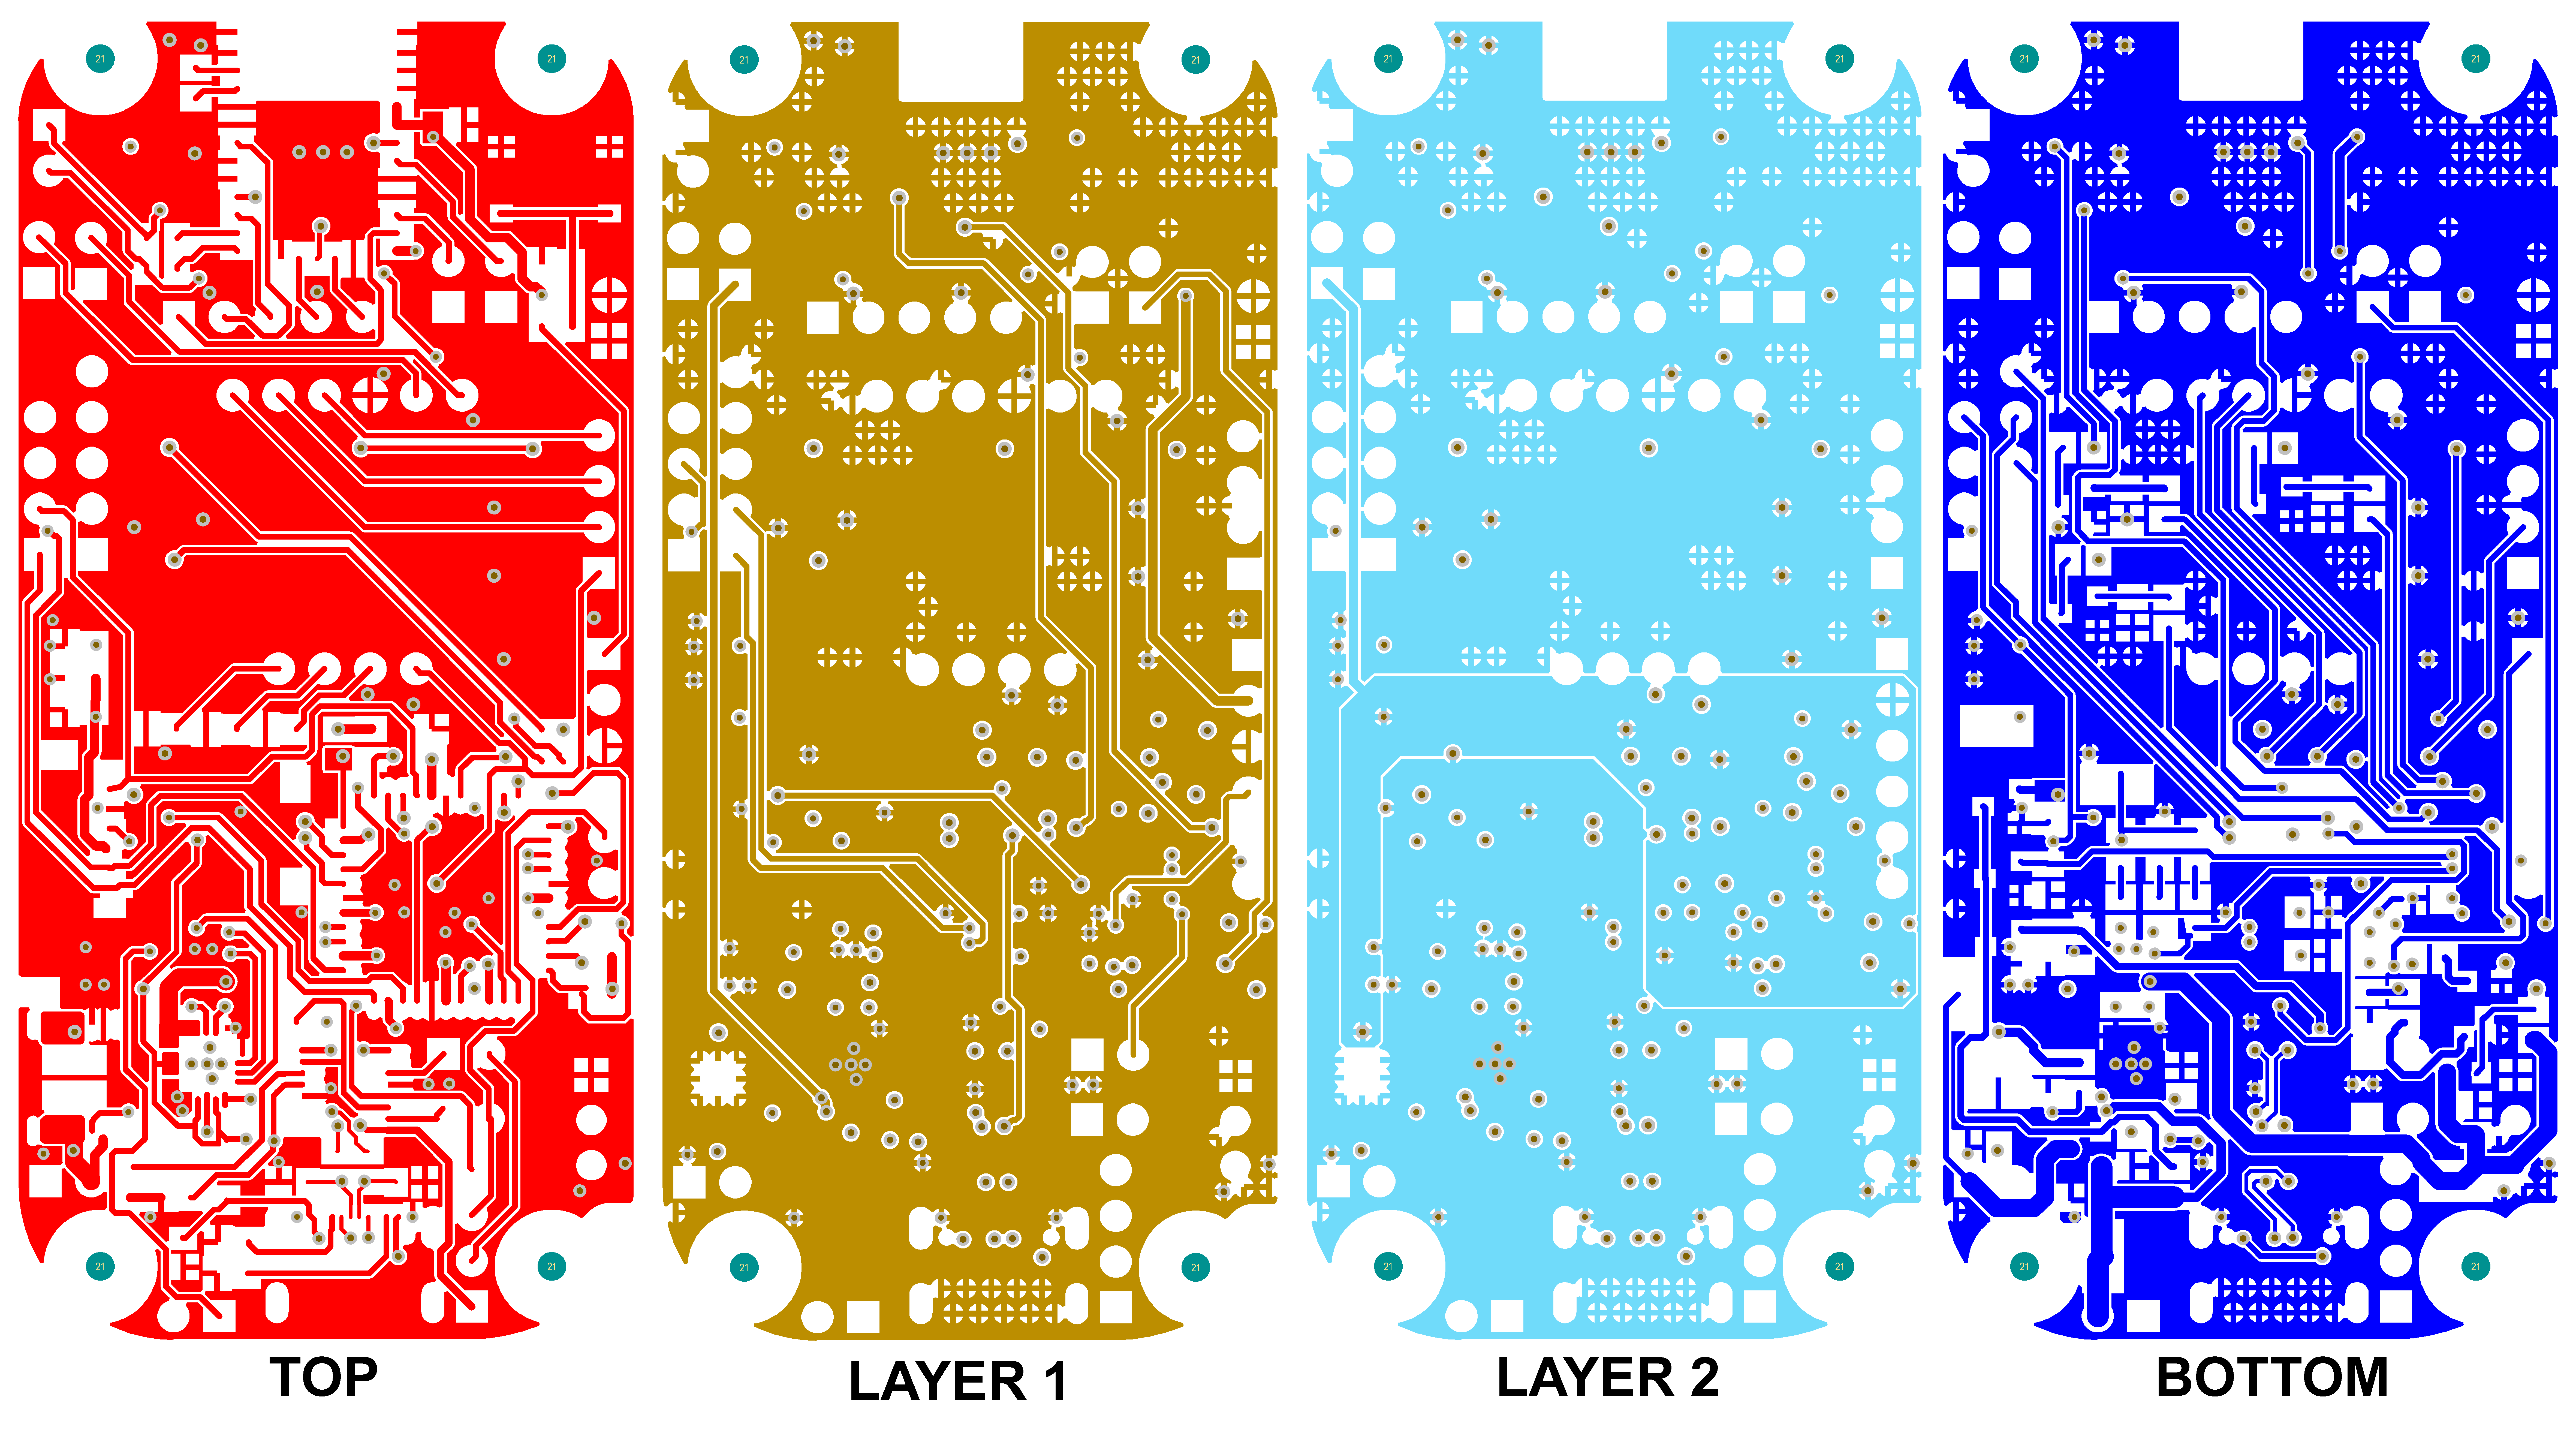
\includegraphics[width=1\linewidth]{../figures/dev-pcb/Couches-layout}
	\caption{Routage des différentes couches}
	\label{fig:couches-layout}
\end{figure}


